\newpage
\section{Analiza problemu}		%2
%Napisać gdzie używa się tego algorytmu
%Opisać sposób działania programu/algorytmu
%Napisać spsoób wykorzystania algorytmu po przez wykonanie przykładu (np. mnożenie macierzy - wykonać ręcznie przykład z mnożeniem macierzy pokazujący jak mnoży się macierz ręcznie)
%Jeśli zadanie zakłada przedstawienie jakiegoś narzędzia (np. git, AI) należy opisać narzędzie

\subsection{Lista}

List używa się przy okazjach, gdy potrzebny jest kontener potrafiący w szybki i prosty sposób modyfikować swoja wielkość i wewnętrzną strukturę, a szybkość dostępu do samych elementów nie jest aż tak ważna.

Lista jest zbiorem połączonych liniowo ze sobą elementów\cite{llistwiki}, gdzie w przypadku tej implementacji, elementy są połączone obustronnie t.zn., każdy element jest połączony z poprzednim i następnym. Dostęp do danego elementu uzyskuje się poprzez enumeracje po kolei wszystkich elementów w liście, aż nie dojdzie się do docelowego. Struktura taka pozwala na łatwe usuwanie i dodawanie elementów - wymaga to tylko zmienienia kilku wskaźników, a nie "przesuwania" całego kontenera. Graficzną reprezentację takiej listy widać na rysunku \ref{fig:list_struct}:

\begin{figure}[H]
	\centering
	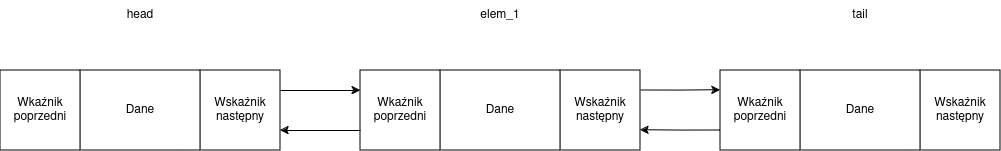
\includegraphics[width=1\textwidth]{images/lista.drawio.png}
	\caption{\centering{Graficzna struktura listy dwukierunkowej}}
	\label{fig:list_struct}
\end{figure}

Strzałki między wskaźnikami na rysunku \ref{fig:list_struct}, symbolizują do jakich miejsc w pamięci wskazują wskaźniki.

Gdybyśmy chcieli dodać jakiś element do listy, proces wyglądałby jak na rys. \ref{fig:}:

\begin{figure}[H]
	\centering
	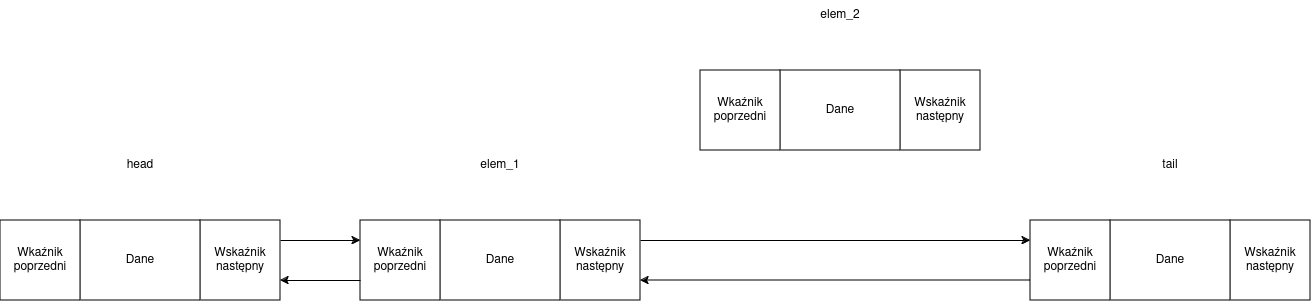
\includegraphics[width=1\textwidth]{images/listadodanie_pre.drawio.png}
	\caption{\centering{Element przed dodaniem do listy}}
	\label{fig:list_add_pre}
\end{figure}

Na rys. \ref{fig:list_add_pre} widać połączenia między elementami listy. \texttt{elem\_2} ma być dodany między \texttt{elem\_1} i \texttt{tail}. 

\begin{figure}[H]
	\centering
	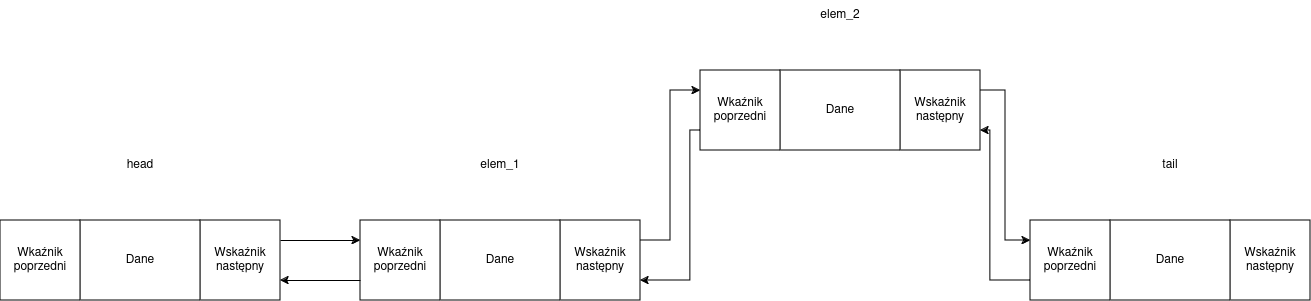
\includegraphics[width=1\textwidth]{images/listadodanie_post.drawio.png}
	\caption{\centering{Element po dodaniu}}
	\label{fig:list_add_post}
\end{figure}

Jak widać z rys. \ref{fig:list_add_post}, wystarczy tylko zmienić adresy na jakie wskazują wskaźniki w danych pozycjach i element zostanie dodany.

\subsection{Git}
Kolejnym konceptem, którym zajmuje się projekt jest narzędzie git\cite{gitsite}. Pozwala ono zarządzać poszczególnymi wersjami projektów. Głównym korzeniem gita jest system commitów, czyli zapisania zmian w pliku w stosunku do commita starszego. To, w połączeniu z jego innymi możliwościami pozwala na tworzenie długich i skomplikowanych osi czasu danych projektów. 

Użycie gita można zademonstrować na prostym przykładzie. Tworzymy katalog a w nim repozytorium, uzywając komendy \texttt{git init}, jak widać na rys. \ref{fig:git_init}.

\begin{figure}[H]
	\centering
	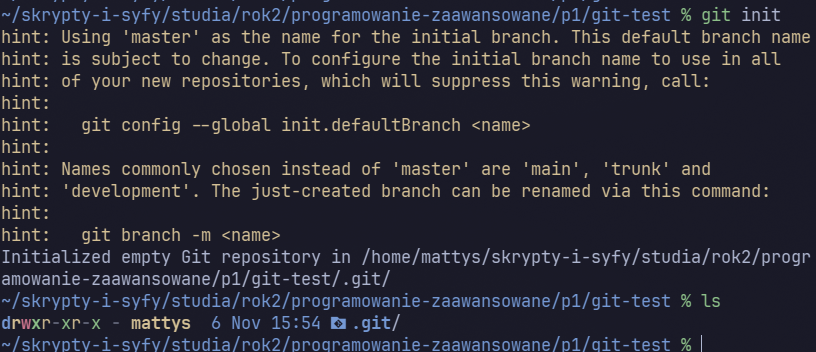
\includegraphics[width=1\textwidth]{images/git_init.png}
	\caption{\centering{Puste repozytorium git}}
	\label{fig:git_init}
\end{figure}

Stwórzmy jakiś plik i dodajmy go do repozytorium. Plik można dodać do repozytorium komendą \texttt{git add}

\begin{figure}[H]
	\centering
	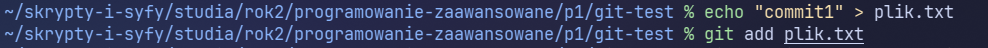
\includegraphics[width=1\textwidth]{images/git_add.png}
	\caption{\centering{Stworznie pliku w repozytorium}}
	\label{fig:git_add}
\end{figure}

Następnie należy scommitować zmiany. 

\begin{figure}[H]
	\centering
	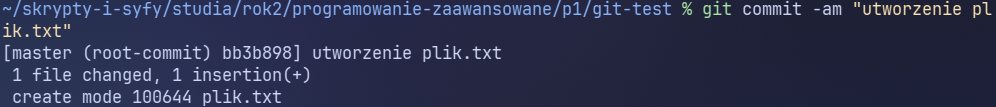
\includegraphics[width=1\textwidth]{images/git_commit1.png}
	\caption{\centering{Commit nr. 1}}
	\label{fig:git_commit1}
\end{figure}

Na rysunku \ref{fig:git_commit1} użyta komenda \texttt{git commit} commituje wszystkie dodane pliki (\texttt{-a}) z jakimś komunikatem (\texttt{-m}).  

\begin{figure}[H]
	\centering
	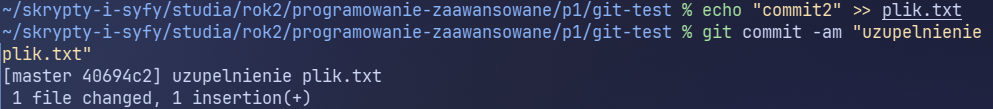
\includegraphics[width=1\textwidth]{images/git_commit2.png}
	\caption{\centering{Commit nr. 2}}
	\label{fig:git_commit2}
\end{figure}

Na rys. \ref{fig:git_commit2}, został utworzony kolejny commit, dodajacy zmiany do \texttt{plik.txt}.

\begin{figure}[H]
	\centering
	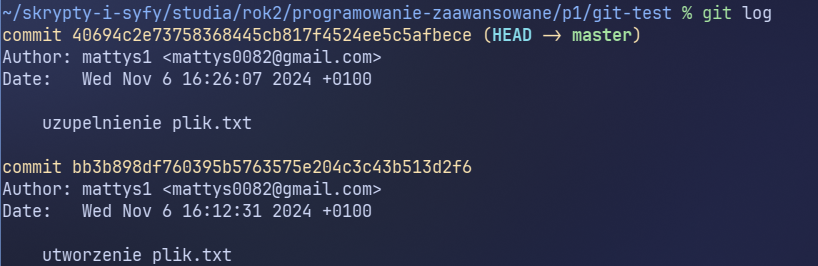
\includegraphics[width=1\textwidth]{images/git_log.png}
	\caption{\centering{Log gita}}
	\label{fig:git_log}
\end{figure}

Jak na rys. \ref{fig:git_log} jest pokazane, używając komendy \texttt{git log}, można wyświetlić log commitów w repozytorium.

\begin{figure}[H]
	\centering
	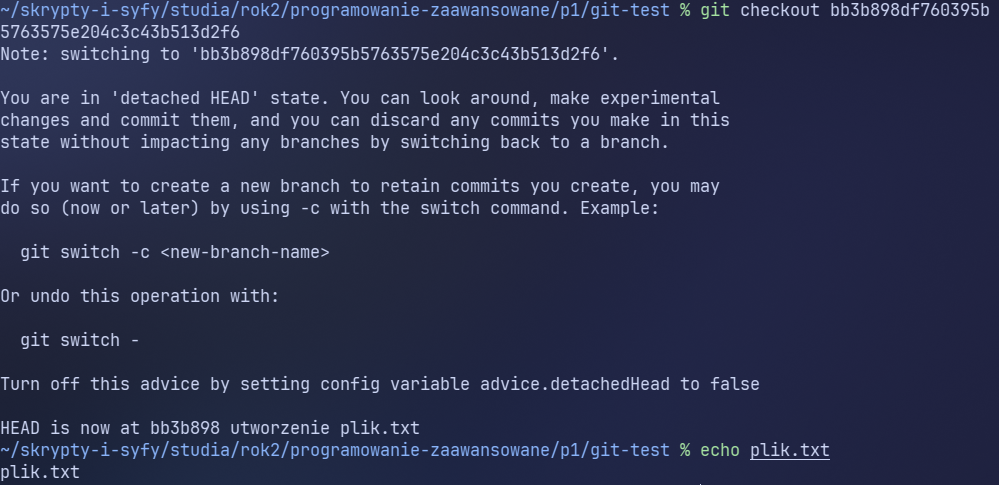
\includegraphics[width=1\textwidth]{images/git_checkout.png}
	\caption{\centering{Demonstracja checkout}}
	\label{fig:git_checkout}
\end{figure}

Jak widać na rys. \ref{fig:git_checkout}, komenda \texttt{git checkout}, pozwala na przejście repozytorium w inny stan, w tym przypadku przechodzi się do commita o danym ID, pokazanym na rys. \ref{fig:git_log}. Jako, że jest to pierwszy commit, nie ma w nim zmian z drugiego.
\subsection{Doxygen}
Doxygen\cite{doxygensite} jest narzędziem automatycznie generującym dokumentację programu z komentarzy w kodzie źródłowym. Potrafi on generować strony HTML, gdzie można dynamicznie nawigować się miedzy rożnymi częściami kodu oraz pliki \LaTeX, które można konwertować na różne, statyczne formaty.
